\documentclass[10pt,journal]{IEEEtran}

% Some very useful LaTeX packages include:
% (uncomment the ones you want to load)





% *** CITATION PACKAGES ***
%
\usepackage{cite}
% cite.sty was written by Donald Arseneau
% V1.6 and later of IEEEtran pre-defines the format of the cite.sty package
% \cite{} output to follow that of the IEEE. Loading the cite package will
% result in citation numbers being automatically sorted and properly
% "compressed/ranged". e.g., [1], [9], [2], [7], [5], [6] without using
% cite.sty will become [1], [2], [5]--[7], [9] using cite.sty. cite.sty's
% \cite will automatically add leading space, if needed. Use cite.sty's
% noadjust option (cite.sty V3.8 and later) if you want to turn this off
% such as if a citation ever needs to be enclosed in parenthesis.
% cite.sty is already installed on most LaTeX systems. Be sure and use
% version 5.0 (2009-03-20) and later if using hyperref.sty.
% The latest version can be obtained at:
% http://www.ctan.org/pkg/cite
% The documentation is contained in the cite.sty file itself.

% *** GRAPHICS RELATED PACKAGES ***
%
\ifCLASSINFOpdf
  \usepackage[pdftex]{graphicx}
  % declare the path(s) where your graphic files are
  \graphicspath{{../Figures/}}
  % and their extensions so you won't have to specify these with
  % every instance of \includegraphics
  % \DeclareGraphicsExtensions{.pdf,.jpeg,.png}
\else
  % or other class option (dvipsone, dvipdf, if not using dvips). graphicx
  % will default to the driver specified in the system graphics.cfg if no
  % driver is specified.
  % \usepackage[dvips]{graphicx}
  % declare the path(s) where your graphic files are
  % \graphicspath{{../eps/}}
  % and their extensions so you won't have to specify these with
  % every instance of \includegraphics
  % \DeclareGraphicsExtensions{.eps}
\fi
% graphicx was written by David Carlisle and Sebastian Rahtz. It is
% required if you want graphics, photos, etc. graphicx.sty is already
% installed on most LaTeX systems. The latest version and documentation
% can be obtained at: 
% http://www.ctan.org/pkg/graphicx
% Another good source of documentation is "Using Imported Graphics in
% LaTeX2e" by Keith Reckdahl which can be found at:
% http://www.ctan.org/pkg/epslatex
%
% latex, and pdflatex in dvi mode, support graphics in encapsulated
% postscript (.eps) format. pdflatex in pdf mode supports graphics
% in .pdf, .jpeg, .png and .mps (metapost) formats. Users should ensure
% that all non-photo figures use a vector format (.eps, .pdf, .mps) and
% not a bitmapped formats (.jpeg, .png). The IEEE frowns on bitmapped formats
% which can result in "jaggedy"/blurry rendering of lines and letters as
% well as large increases in file sizes.
%
% You can find documentation about the pdfTeX application at:
% http://www.tug.org/applications/pdftex





% *** MATH PACKAGES ***
%
\usepackage{amsmath}
\DeclareMathOperator*{\argmin}{argmin}
\DeclareMathOperator*{\argmax}{argmax}
% A popular package from the American Mathematical Society that provides
% many useful and powerful commands for dealing with mathematics.
%
% Note that the amsmath package sets \interdisplaylinepenalty to 10000
% thus preventing page breaks from occurring within multiline equations. Use:
\interdisplaylinepenalty=2500
% after loading amsmath to restore such page breaks as IEEEtran.cls normally
% does. amsmath.sty is already installed on most LaTeX systems. The latest
% version and documentation can be obtained at:
% http://www.ctan.org/pkg/amsmath





% *** SPECIALIZED LIST PACKAGES ***
%
%\usepackage{algorithmic}
% algorithmic.sty was written by Peter Williams and Rogerio Brito.
% This package provides an algorithmic environment fo describing algorithms.
% You can use the algorithmic environment in-text or within a figure
% environment to provide for a floating algorithm. Do NOT use the algorithm
% floating environment provided by algorithm.sty (by the same authors) or
% algorithm2e.sty (by Christophe Fiorio) as the IEEE does not use dedicated
% algorithm float types and packages that provide these will not provide
% correct IEEE style captions. The latest version and documentation of
% algorithmic.sty can be obtained at:
% http://www.ctan.org/pkg/algorithms
% Also of interest may be the (relatively newer and more customizable)
% algorithmicx.sty package by Szasz Janos:
% http://www.ctan.org/pkg/algorithmicx




% *** ALIGNMENT PACKAGES ***
%
\usepackage{array}
% Frank Mittelbach's and David Carlisle's array.sty patches and improves
% the standard LaTeX2e array and tabular environments to provide better
% appearance and additional user controls. As the default LaTeX2e table
% generation code is lacking to the point of almost being broken with
% respect to the quality of the end results, all users are strongly
% advised to use an enhanced (at the very least that provided by array.sty)
% set of table tools. array.sty is already installed on most systems. The
% latest version and documentation can be obtained at:
% http://www.ctan.org/pkg/array


% IEEEtran contains the IEEEeqnarray family of commands that can be used to
% generate multiline equations as well as matrices, tables, etc., of high
% quality.




% *** SUBFIGURE PACKAGES ***
%\ifCLASSOPTIONcompsoc
%  \usepackage[caption=false,font=normalsize,labelfont=sf,textfont=sf]{subfig}
%\else
%  \usepackage[caption=false,font=footnotesize]{subfig}
%\fi
% subfig.sty, written by Steven Douglas Cochran, is the modern replacement
% for subfigure.sty, the latter of which is no longer maintained and is
% incompatible with some LaTeX packages including fixltx2e. However,
% subfig.sty requires and automatically loads Axel Sommerfeldt's caption.sty
% which will override IEEEtran.cls' handling of captions and this will result
% in non-IEEE style figure/table captions. To prevent this problem, be sure
% and invoke subfig.sty's "caption=false" package option (available since
% subfig.sty version 1.3, 2005/06/28) as this is will preserve IEEEtran.cls
% handling of captions.
% Note that the Computer Society format requires a larger sans serif font
% than the serif footnote size font used in traditional IEEE formatting
% and thus the need to invoke different subfig.sty package options depending
% on whether compsoc mode has been enabled.
%
% The latest version and documentation of subfig.sty can be obtained at:
% http://www.ctan.org/pkg/subfig




% *** FLOAT PACKAGES ***
%
%\usepackage{fixltx2e}
% fixltx2e, the successor to the earlier fix2col.sty, was written by
% Frank Mittelbach and David Carlisle. This package corrects a few problems
% in the LaTeX2e kernel, the most notable of which is that in current
% LaTeX2e releases, the ordering of single and double column floats is not
% guaranteed to be preserved. Thus, an unpatched LaTeX2e can allow a
% single column figure to be placed prior to an earlier double column
% figure.
% Be aware that LaTeX2e kernels dated 2015 and later have fixltx2e.sty's
% corrections already built into the system in which case a warning will
% be issued if an attempt is made to load fixltx2e.sty as it is no longer
% needed.
% The latest version and documentation can be found at:
% http://www.ctan.org/pkg/fixltx2e


%\usepackage{stfloats}
% stfloats.sty was written by Sigitas Tolusis. This package gives LaTeX2e
% the ability to do double column floats at the bottom of the page as well
% as the top. (e.g., "\begin{figure*}[!b]" is not normally possible in
% LaTeX2e). It also provides a command:
%\fnbelowfloat
% to enable the placement of footnotes below bottom floats (the standard
% LaTeX2e kernel puts them above bottom floats). This is an invasive package
% which rewrites many portions of the LaTeX2e float routines. It may not work
% with other packages that modify the LaTeX2e float routines. The latest
% version and documentation can be obtained at:
% http://www.ctan.org/pkg/stfloats
% Do not use the stfloats baselinefloat ability as the IEEE does not allow
% \baselineskip to stretch. Authors submitting work to the IEEE should note
% that the IEEE rarely uses double column equations and that authors should try
% to avoid such use. Do not be tempted to use the cuted.sty or midfloat.sty
% packages (also by Sigitas Tolusis) as the IEEE does not format its papers in
% such ways.
% Do not attempt to use stfloats with fixltx2e as they are incompatible.
% Instead, use Morten Hogholm'a dblfloatfix which combines the features
% of both fixltx2e and stfloats:
%
% \usepackage{dblfloatfix}
% The latest version can be found at:
% http://www.ctan.org/pkg/dblfloatfix




%\ifCLASSOPTIONcaptionsoff
%  \usepackage[nomarkers]{endfloat}
% \let\MYoriglatexcaption\caption
% \renewcommand{\caption}[2][\relax]{\MYoriglatexcaption[#2]{#2}}
%\fi
% endfloat.sty was written by James Darrell McCauley, Jeff Goldberg and 
% Axel Sommerfeldt. This package may be useful when used in conjunction with 
% IEEEtran.cls'  captionsoff option. Some IEEE journals/societies require that
% submissions have lists of figures/tables at the end of the paper and that
% figures/tables without any captions are placed on a page by themselves at
% the end of the document. If needed, the draftcls IEEEtran class option or
% \CLASSINPUTbaselinestretch interface can be used to increase the line
% spacing as well. Be sure and use the nomarkers option of endfloat to
% prevent endfloat from "marking" where the figures would have been placed
% in the text. The two hack lines of code above are a slight modification of
% that suggested by in the endfloat docs (section 8.4.1) to ensure that
% the full captions always appear in the list of figures/tables - even if
% the user used the short optional argument of \caption[]{}.
% IEEE papers do not typically make use of \caption[]'s optional argument,
% so this should not be an issue. A similar trick can be used to disable
% captions of packages such as subfig.sty that lack options to turn off
% the subcaptions:
% For subfig.sty:
% \let\MYorigsubfloat\subfloat
% \renewcommand{\subfloat}[2][\relax]{\MYorigsubfloat[]{#2}}
% However, the above trick will not work if both optional arguments of
% the \subfloat command are used. Furthermore, there needs to be a
% description of each subfigure *somewhere* and endfloat does not add
% subfigure captions to its list of figures. Thus, the best approach is to
% avoid the use of subfigure captions (many IEEE journals avoid them anyway)
% and instead reference/explain all the subfigures within the main caption.
% The latest version of endfloat.sty and its documentation can obtained at:
% http://www.ctan.org/pkg/endfloat
%
% The IEEEtran \ifCLASSOPTIONcaptionsoff conditional can also be used
% later in the document, say, to conditionally put the References on a 
% page by themselves.




% *** PDF, URL AND HYPERLINK PACKAGES ***
%
%\usepackage{url}
% url.sty was written by Donald Arseneau. It provides better support for
% handling and breaking URLs. url.sty is already installed on most LaTeX
% systems. The latest version and documentation can be obtained at:
% http://www.ctan.org/pkg/url
% Basically, \url{my_url_here}.




% *** Do not adjust lengths that control margins, column widths, etc. ***
% *** Do not use packages that alter fonts (such as pslatex).         ***
% There should be no need to do such things with IEEEtran.cls V1.6 and later.
% (Unless specifically asked to do so by the journal or conference you plan
% to submit to, of course. )

% Other packages
\usepackage{amssymb}
\usepackage{mathtools}


% correct bad hyphenation here
\hyphenation{op-tical net-works semi-conduc-tor}


\begin{document}
%
% paper title
% Titles are generally capitalized except for words such as a, an, and, as,
% at, but, by, for, in, nor, of, on, or, the, to and up, which are usually
% not capitalized unless they are the first or last word of the title.
% Linebreaks \\ can be used within to get better formatting as desired.
% Do not put math or special symbols in the title.
\title{Learning an Optimal Policy for Police Resource Allocation on Freeways}
%
%
% author names and IEEE memberships
% note positions of commas and nonbreaking spaces ( ~ ) LaTeX will not break
% a structure at a ~ so this keeps an author's name from being broken across
% two lines.
% use \thanks{} to gain access to the first footnote area
% a separate \thanks must be used for each paragraph as LaTeX2e's \thanks
% was not built to handle multiple paragraphs
%

\author{Brian~Jackson,
        Taylor~Howell,
        and~Ola~Shorinwa% <-this % stops a space
\thanks{Department of Mechanical Engineering, Stanford University}}

% note the % following the last \IEEEmembership and also \thanks - 
% these prevent an unwanted space from occurring between the last author name
% and the end of the author line. i.e., if you had this:
% 
% \author{....lastname \thanks{...} \thanks{...} }
%                     ^------------^------------^----Do not want these spaces!
%
% a space would be appended to the last name and could cause every name on that
% line to be shifted left slightly. This is one of those "LaTeX things". For
% instance, "\textbf{A} \textbf{B}" will typeset as "A B" not "AB". To get
% "AB" then you have to do: "\textbf{A}\textbf{B}"
% \thanks is no different in this regard, so shield the last } of each \thanks
% that ends a line with a % and do not let a space in before the next \thanks.
% Spaces after \IEEEmembership other than the last one are OK (and needed) as
% you are supposed to have spaces between the names. For what it is worth,
% this is a minor point as most people would not even notice if the said evil
% space somehow managed to creep in.



% The paper headers
\markboth{Machine Learning (CS229), December 2017}%
{Shell \MakeLowercase{\textit{et al.}}: Bare Demo of IEEEtran.cls for IEEE Journals}
% The only time the second header will appear is for the odd numbered pages
% after the title page when using the twoside option.
% 
% *** Note that you probably will NOT want to include the author's ***
% *** name in the headers of peer review papers.                   ***
% You can use \ifCLASSOPTIONpeerreview for conditional compilation here if
% you desire.




% If you want to put a publisher's ID mark on the page you can do it like
% this:
%\IEEEpubid{0000--0000/00\$00.00~\copyright~2015 IEEE}
% Remember, if you use this you must call \IEEEpubidadjcol in the second
% column for its text to clear the IEEEpubid mark.



% use for special paper notices
%\IEEEspecialpapernotice{(Invited Paper)}




% make the title area
\maketitle

% As a general rule, do not put math, special symbols or citations
% in the abstract or keywords.
\begin{abstract}
Anomaly detection is a well-studied area within computer science and artificial intelligence given its extremely useful applications in surveillance, driver assistance, and navigation. In this project, we apply a fundamental anomaly detection algorithm using Principal Component Analysis (PCA) and a Mixture of Gaussians model to the NGSIM highway dataset of real-world vehicle trajectories in congested traffic conditions. After identifying the feature distributions for anomalous drivers we apply these distributions to a simulator to learn an optimal policy for police allocation to apprehend anomalous vehicles. We formulate the police allocation problem as a Markov Decision Process (MDP) and learn the optimal using using reinforcement learning (RL). We are successfully able to learn a policy that chooses to only deploy vehicles when the expected reward is above a certain threshold. 
\end{abstract}

% Note that keywords are not normally used for peerreview papers.
\begin{IEEEkeywords}
EM algorithm, Principal Component Analysis, Markov Decision Process, machine learning, reinforcement learning
\end{IEEEkeywords}

% For peer review papers, you can put extra information on the cover
% page as needed:
% \ifCLASSOPTIONpeerreview
% \begin{center} \bfseries EDICS Category: 3-BBND \end{center}
% \fi
%
% For peerreview papers, this IEEEtran command inserts a page break and
% creates the second title. It will be ignored for other modes.
\IEEEpeerreviewmaketitle



\section{Introduction}
\IEEEPARstart{T}{raffic} accidents account for a majority of deaths annually in the United States. The purpose of this project is to develop a framework for identifying ``anomalous'' drivers on the freeway and optimally allocating police resources to apprehend and cite these drivers. In the context of this project, anomalous drivers may or may not be breaking laws such as speeding, tailgating, or weaving in and out of traffic; however, if their driving style is significantly different than the rest of the cars around them, some benefit may be had in identifying the underlying cause of their observed behavior. For instance, it may be possible to identify drunk or impaired drivers, distracted drivers, or people who have stolen a car or kidnapped someone. Surveillance systems that automatically detect anomalous drivers can act as useful tools to help law enforcement agencies more efficiently sift through the thousands of drivers on the road and focus on ones that ``stand out.''

Once these drivers are identified, the allocation of scarce resources (in this case, highway patrol vehicles) to optimally apprehend suspicious or unlawful activity is yet another challenge. In this project, we aim to solve both of these problems, namely: identification of anomalous drivers, and finding an optimal policy for allocating police resources. The first problem is solved by learning a mixture-of-Gaussians model from a data set taken from actual highway data. The second problem is framed as a Markov Decision Process (MDP) and solved using reinforcement learning (RL) techniques. 

The problem of detecting anomalous driver is a well-studied problem given its valuable applications in surveillance, crisis prevention, driver assistance, and navigation. \cite{chandola2009anomaly} gives an overview of various approaches to anomalous behavior detection, which are categorized into the following classes: classification-based, parametric or non-parametric statistical, nearest neighbor-based, clustering-based, spectral techniques, and information theoretic. Many studies have taken a similar approach the one used in the current project. Notably, Morris and Trivedi \cite{morris2008survey} propose an algorithm for extracting trajectory information from camera data, compressing the feature subspace using Principal Component Analysis (also used in the current project), and then classified using a variety of unsupervised learning techniques including K-means, fuzzy-C-means, and neural networks. New trajectories are assigned a score rating how anomalous they are, based upon the distance to the nearest cluster. Other approaches have included support-vector machines (SVMs) \cite{piciarelli2008trajectory}, Hidden-Markov Models clustered using K-means \cite{suzuki2007learning}, and semi-supervised learning \cite{sillito2008semi}. The field of anomaly detection is a broad and very active area of research, and presenting any sort of in-depth analysis of the various approaches is beyond the scope of this class project. However, based on the cited papers, SVM techniques are advantageous given their computation efficiency, while the more traditional approach is advantageous given that it builds a distribution modeling ``typical'' driver behavior. The semi-supervised learning approach showed promising results but requires human-in-the-loop training and is susceptible to undetected anomalies making it into the model. It seems current state-of-the-art techniques like the one presented by An and Cho \cite{an2015variational} use deep-learning-based autoencoders, that reduce feature dimensionality and increase abstract generalization. An and Cho present an algorithm for variation autoencoders that (VAE) that combine deep autoencoders with variational inference. Additionally, since it is a generative model, it can also be used to derive the underlying model and analyze the underlying cause of the anomaly.

Resource allocation is also a fairly well-studied field, and the topic of police allocation in particular has received some attention. However, applying state-of-the-art decision making algorithms to police allocation is very limited \cite{locationallocation}, and typically based on optimizing deployment location rather than deciding whether or not to deploy limited resources. Our project therefore seems to be a novel application of decision-making processes to learning an optimal policy for deploying police in an uncertain environment with variable rewards. 

\section{Methodology}
The project is divided into three principal components: 1) preprocessing: analyzing and compressing real-world highway-driving data, 2) anomaly detection: identifying anomalous drivers from the dataset, and 3) the MDP: learning an optimal policy for deploying police resources to cite anomalous drivers and maximize ticket revenue. We assume that it's possible to detect anomalous driving behavior that corresponds with traffic offenses on freeways and that it's possible to indirectly make the freeway safer by maximizing ticket revenue. We will model highway driving behavior as a mixture of Gaussians and characterize atypical driving behavior as lying outside the modeled distributions. We will be working with the NGSIM highway data set, which tracks vehicle trajectories in congested morning traffic along a half mile section of Highway 101. We will use the EM algorithm to train the model with features from these driving trajectories.

\subsection*{Data Processing} \label{data}
We are using real-world driver data from the NGSIM US-101 dataset. The data was captured using a set of cameras set atop a 36-story building. This data has been processed into vehicle trajectories that track individual vehicles and report features such as width, length, velocity, position, lane, etc. However, the original trajectory data contains significant noise in the position, velocity, and acceleration estimates. We are using data that has been post-processed by members of SISL (Stanford Intelligent Systems Laboratory), which improves state estimates using a Kalman filter. The resulting data data consists of 45 minutes of vehicle trajectories, including about 6000 unique vehicle trajectories. From this filtered data we have constructed a training set consisting of averages over 15-second time intervals with 5 second spacing, resulting in about 64,000 examples. 

Each of these examples contains 6 features: average velocity, average acceleration, maximum velocity, number of lane changes, average deviation from lane centers, and standard deviation from lane center. The velocity, acceleration, and deviation from lane center were all given by the filtered dataset. The averages, maximums and standard deviation were taken over the 15 second time window of interest. The number of lane changes was determined by counting the number of times the lane deviation varied by more than a fixed threshold in a given time step (in either direction). The resulting features should give a decent depiction of driver behavior over a moderate time window and be sufficient to identify anomalous behavior. 

\subsection*{Anomaly Detection}
\subsubsection{EM Algorithm}
We assumed that each example came from a joint distribution $p(x,z)=p(x|z)p(z)$ consisting of four Gaussians. Thus, each $x^{(i)}$ was obtained by randomly choosing $z^{(i)}\in\left\{1,2,...,k\right\}$ and then sampling $x^{(i)}$ from the corresponding Gaussian distribution. We intend to learn the parameters of the joint distribution $p(x,z;\theta)$ for the training examples where $z^{(i)}$ represents the latent variables and $\theta=\left\{\phi,\mu,\Sigma\right\}$. Finding a closed form solution for the maximum likelihood estimates of $\theta$ is difficult; hence, we used the EM algorithm for estimating $\theta$. The EM algorithm works by constructing a lower bound on the log-likelihood of the training set $\ell(\theta)$ before optimizing the lower bound. The algorithm is given below.\\
\indent E-step: For each i,\\
$$\displaystyle Q_{i}(z^{(i)}) \coloneqq p(z^{(i)}|x^{(i)};\theta)$$
\indent M-step: Set \\
$$\displaystyle \theta \coloneqq \argmin_{\theta} {\sum_{i}^m\sum_{z^{(i)}} Q_{i}(z^{(i)})\log\dfrac{p(x^{(i)},z^{(i)};\theta)}{Q_{i}(z^{(i)})}}$$
We use the estimated parameters in fitting a Mixture of Gaussians to the NGSIM data set and identify outliers using a threshold $p(x)<0.0025$. 

\subsubsection{Principal Component Analysis}
We used principal component analysis as a dimensionality reduction algorithm to map the extracted features to different feature spaces ranging from sizes 2 to 5. The first $k$ principal components of the data were selected to maximize the variance of the projections where the first principal component satisfies the optimization problem:
$$\displaystyle u \coloneqq \argmax_{u:u^{T}u=1}{\dfrac{1}{m}\sum_{i=1}^{m}(x^{(i)^{T}}u)^{2}}$$

We apply the EM algorithm to each of the resulting feature spaces to obtain a model for classifying anomalous drivers. The features of the anomalous drivers flagged by each model was analyzed to evaluate the performance of each model.

\subsection*{The MDP}
We have formulated the task of allocating police resources on freeways as a discounted infinite-horizon Markov decision process.

\subsubsection*{MDP Formulation}
The state is defined by 2 variables: the police state and the driver state. The police state is the vector $P = [p_1 \dots p_{n_p}] \in \mathbb{Z}^{n_p}$ of police car states $p \in \{0,1,...,p_{max}\}$. Each integer $p_i$ represents the number of time steps until the police car $i$ is again available for allocation. $p_i=0$ indicates that police $i$ is ready for allocation. After being allocated, $p_i = p_{max}$ and decrements by 1 each time step. The driver state is the vector $D = [d_1\dots d_{n_d}]\in \mathbb{Z}^{n_d}$ of driver states $d \in \{1,...,d_{max}\}$. The integer values $d_j$ correspond to the state of the anomalous vehicle $j$, defined as follows:

\begin{table}[h]
\centering
\begin{tabular}[h]{c c l l}
\firsthline
d & Reward & Description & Conditions \\
\hline
1 & 50 & No citation  & Not 2 or 3 \\
2 & 100 & Speeder & Speed $>$ 17 m/s \\
3 & 150 & Weaver & \# lane changes $>$ 3 \\
4 & 250 & Both & Both 2 \& 3 \\
\lasthline 
\end{tabular}
\label{tab:citations}
\caption{Definition of anomalous vehicle states}
\end{table}

\noindent The size of the state space is $(p_{max})^{n_p} \times (d_{max})^{n_d}$. For our final solution, we set $n_p = 2, n_d = 4,$, $p_{max} = 5$, and $d_{max} = 4$. 

The action space defines the allocation of police cars in $P$. The action $a = \{0,1,\dots,n_p\} \in \mathbb{Z}$ corresponds to the number of citations to deliver. It is assumed that the vehicles in D with the highest reward will be cited.

The rewards are deterministically assigned: each vehicle state $p_j$ is assigned a particular reward, as shown in Table \ref{tab:citations}. If $a>0$, the resulting reward is the sum of the $a$ highest rewards corresponding to states in $D$. If $a>0$ and $p_i \neq 0, \forall p_i \in P$ (no police available), then a penalty of -100 was assigned.

\subsubsection*{Scene simulation}
Since the NGSIM data set only gives us a finite amount of experience, we created a simulation that can sample from distributions based upon the NGSIM data set. The simulator maintains an internal ``scene'' of anomalous vehicles. A scene contains 10 vehicles, specified by the features listed in section \ref{data}, in addition to a unique vehicle ID and a time stamp. The time stamp of each vehicle is decremented at each time step and vehicles with negative time stamps are removed from the scene. The features are sampled from independent distributions. The authors acknowledge that in reality the anomalous drivers are more likely to belong to a multivariate distribution that encodes dependence between different features, such as average velocity and number of lane changes, but for simplicity these features were assumed to be independent, and the resulting samples will consequently not be guaranteed to be anomalous. However, only $n_d$ of the 10 vehicles are selected from each scene, according to highest reward. This is a fair assumption since it would clearly be sub-optimal to issue a citation to a vehicle known to yield less reward (given our previous assumption that the rewards are deterministic). At each time step, new vehicles are added to keep the total number of vehicles in each scene constant. New vehicles were always initialized with a time stamp of $p_{max}$ (described above). The time stamp was included with the purpose of modeling the fact that drivers can only be observed for a fixed amount of time and that the police only have a finite amount of time to decide whether or not to apprehend the vehicle. After adding the new vehicles, they are assigned a state value as a deterministic function of their features (actually, only maximum velocity and number of lane changes), according to the conditions listed in Table \ref{tab:citations}. The distribution of vehicle state values used in the simulation is shown in Figure \ref{fig:statehist}. It should be noted that the threshold for speeding (17 m/s, or 38 mph) is lower than the actual speed limit (65 mph). Since the data was recorded during heavily congested morning traffic, the speed limit was artificially lowered so that about half of the anomalous drivers were speeding (as shown by the distribution in Figure \ref{fig:statehist}). 

\begin{figure}[!t]
\centering
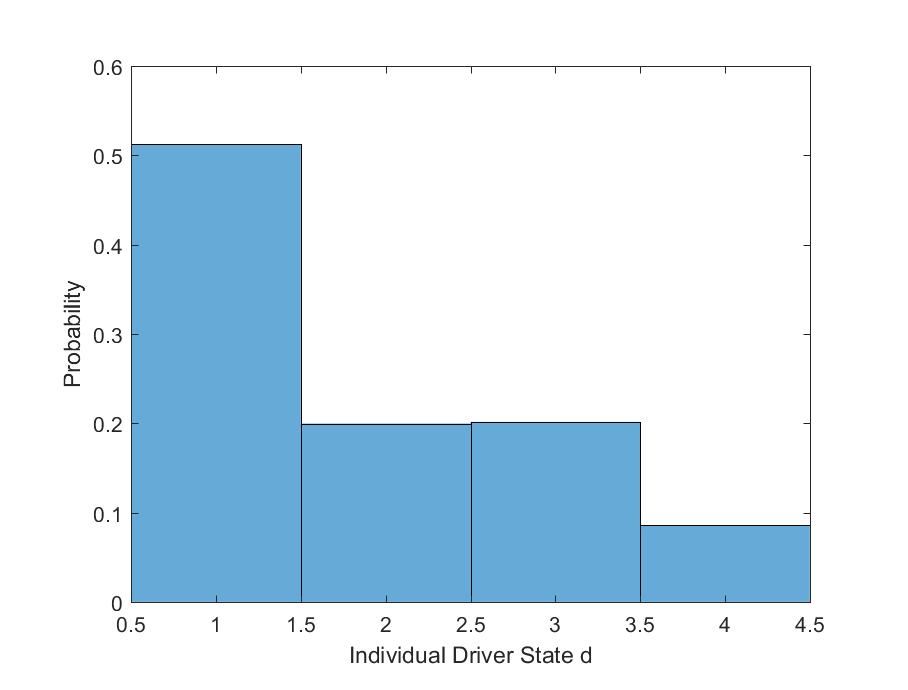
\includegraphics[width=2.5in]{Figures/DriverStateHistogram}
\caption{Distribution of individual vehicle states used by simulation}
\label{fig:statehist}
\end{figure}

At each time step, the simulator accepts a state/action tuple and returns the subsequent state and resulting reward. Based on the input state and action, it issues citations to the vehicles in $D$ with the highest reward and removes them from the scene. It then updates the scene by decrementing the time stamps and adding new vehicles.  

\subsubsection*{Solving the MDP}
We use model-based reinforcement learning techniques to find an optimal policy for the MDP. The agent gains experience by interacting with the simulator for $n$ time steps before updating the transition $T$ and reward $R$ models using maximum likelihood estimates. Asynchronous value iteration is performed on the Bellman equation (Eq. \ref{eq:bellman}) until convergence.

\begin{equation} \label{eq:bellman}
	U^*(s) \coloneqq \max_{a}{\bigl(R(s,a)+\gamma\sum_{s'}T(s'|s,a)U^*(s')\bigr)}
\end{equation}

An update to the value function was assumed to have converged when $||U_k-U_{k-1}|| < 0.005$. The learning procedure was repeated until 10 consecutive updates of the MDP model and the value function converged on the first iteration. The optimal policy $\pi^{*}(s)$ was obtained from the optimal value function.

\begin{equation*} \label{eq:bellmanpolicy}
	\pi^*(s) \coloneqq \argmax_{a}{\bigl(R(s,a)+\gamma\sum_{s'}T(s'|s,a)U^*(s')\bigr)}
\end{equation*}

To evaluate the optimal policy, we calculate the cumulative rewards per time step when following the optimal policy and compare it against the cumulative rewards per time step following a blind policy that randomly assigns police vehicles to apprehend offending drivers and an always-allocate policy that assigns the maximum number of available police vehicles.


\section{Results}
\subsection{Anomaly Detection}
New feature sets of sizes ranging from 2 to 5 were constructed from the highway data set using PCA. These feature sets were evaluated against the baseline model consisting of six features. The anomaly detection model was created by fitting four Gaussians to each feature set. Anomalous drivers were identified using a threshold $p(x)<0.0025$. Table  \ref{tab:NumDrivers} shows the percentage of anomalous drivers flagged by each model. The number of anomalous drivers decreases with the size of the feature space.The baseline model flagged about 30\% (1780) of drivers as atypical while the two-feature set model identified a substantially lower percentage of atypical drivers, 1\% (15). The three-feature and four-feature models classified about 4\% (220) and 6\% (323) of drivers as atypical respectively.

\begin{figure}[!t]
	\centering
    \includegraphics[width=0.9\columnwidth]{"Figures/num_drivers"}
	\caption{Percentage of Anomalous Drivers for each model}
    \label{fig:NumDrivers}
\end{figure}

\begin{table}[!t]
\centering
\begin{tabular}[h]{c | c}
\hline
Size of feature space & Percentage of anomalous drivers (\%) \\
\hline
2 & 0.249 \\
3 & 3.648 \\
4 & 5.356 \\
5 & 29.514 \\
\hline
\end{tabular}
\caption{Percentage of Anomalous Drivers for each model}
\label{tab:NumDrivers}
\end{table}



The features of the flagged drivers were analyzed to further evaluate the effects of dimensionality reduction using PCA. Figure \ref{fig:NumLanes} shows the histogram of the number of lane changes of outliers identified by the two-feature and baseline models. The two-feature model flags drivers having a high number of lane changes with high probability compared to the baseline model. The drivers with zero lane changes which were classified as anomalous exceeded the acceptable limits on other features.

\begin{figure}[!t]
	\centering
    \includegraphics[width=0.9\columnwidth]{"Figures/num_lanes"}
    \caption{Histogram of number of lane changes of anomalous drivers for two-feature and baseline models}
    \label{fig:NumLanes}
\end{figure}

Figure \ref{fig:AvgAccel} shows the normalized histograms of the average acceleration of anomalous drivers identified by the two-feature and baseline models. The two-feature model performs considerably well in identifying drivers with extreme accelerations, flagging such drivers as anomalous with a high probability. In contrast, drivers with acceptable accelerations have a higher probability of being flagged anomalous by the baseline model compared with drivers with extreme accelerations. The results show that the application of PCA helped reduce the susceptibility of the model to noisy observations, ultimately improving the accuracy of the anomaly detection algorithm. The PCA model retained the valuable variations among the feature attributes while discarding noisy variations which resulted in the model flagging a lower percentage of drivers as anomalous. The application of PCA also provided computational benefits by reducing the size of the feature sets. Such computational benefits scale with the size of the training set.

\begin{figure}[!t]
	\centering
    \includegraphics[width=0.9\columnwidth]{"Figures/avg_acceleration"}
	\caption{Histogram of average acceleration of anomalous drivers for two-feature and baseline models}
    \label{fig:AvgAccel}
\end{figure}

The simulator for the MDP generates new anomalous vehicles by sampling from independent distributions over each feature. The distributions over these features were created from the anomalous drivers identified by the two-feature model. The normalized histograms of the features are multi-modal; hence, the features could not be modeled as a unimodal Gaussian distribution. We estimated the distribution using a normal kernel distribution with different bandwidths. The bandwidth parameter controls the smoothness of the probability density curve. Figure \ref{fig:KernDistri} shows the fitted probability distributions over the features for different bandwidths. The default bandwidth parameter shown in the figure results from optimizing the mean integrated square error. A bandwidth parameter of one provided better estimations of the probability density curves of the number of lane changes, average velocity, and maximum velocity, showing the major peaks in the probability density curve for these features. The kernel distribution using the theoretically optimized bandwidth parameter provided a better estimate of the probability density curve of the average acceleration and was thus used by the simulator.

\begin{figure}[!t]
	\centering
    \includegraphics[width=1.1\columnwidth]{"Figures/distribution_drivers"}
    \caption{Kernel distribution over the (a)number of lane changes, (b)average velocity, and (c)maximum velocity and (d)average acceleration for different bandwidths}
    \label{fig:KernDistri}
\end{figure}

\subsection{Optimal Policy}
For the simple MDP with 1 police and 2 anomalous drivers, solving for the optimal policy took 2135.18 seconds, converging after 21,000 epochs (100 steps of experience per epoch). An $\epsilon$-greedy strategy was used with $\epsilon$ = 0.1 and a discount factor $\gamma$ = 0.9. For any state with no police to allocate (i.e., $\sum_{i=1}^{n_p} p_i = 0$) the police learned to do nothing (i.e., action = 0) which is optimal since taking any other action in this state will result in a negative reward. To better understand the policy, we examine the policy at critical states where police are available for allocation (i.e., $p_i$ = 0). For these states, we find that there is some threshold such that drivers with low reward values are not cited. We found that drivers with $d_i < x$ were not cited. This demonstrates that our agent was able to learn an intelligent policy that enables it to delay immediate reward for greater future reward. We compare the optimal policy with a random-allocation policy (if $\sum_{i=1}^{n_p} p_i > 0$ then a random number of available police are allocated, else no police are allocated) and always-allocate policy (number of police allocated = $\sum_{i=1}^{n_p}$. Because we are interested in efficiently allocating resources, we compare the average cumulative reward per allocation for each policy for a 1000 step episode for 5 trials and then average the results. The results of the learned optimal policy during training versus the "expert" policies are shown in Figure \ref{fig:learningCurve}.\\

\begin{table}                        
\centering                           
\begin{tabular}{|c|c|c|c|c|c|c|}
\firsthline
\multicolumn{3}{|c|}{\textbf{State}} & \textbf{Value} & \multicolumn{3}{c|}{\textbf{Policy}} \\
\hline 
$d_{1}$ & $d_2$ & $p_1$ & U* & Optimal & Always & Random\\
\hline
    1 & 1 & 0 & 333.209 & 0 & 1 & 0 \\
    \hline
    2 & 1 & 0 & 341.488 & 0 & 1 & 0 \\
    \hline
    3 & 1 & 0 & 372.812 & 1 & 1 & 1 \\
    \hline
    4 & 1 & 0 & 454.712 & 1 & 1 & 1 \\
    \hline
    2 & 2 & 0 & 341.113 & 0 & 1 & 0 \\
    \hline
    3 & 2 & 0 & 377.063 & 1 & 1 & 1 \\
    \hline
    4 & 2 & 0 & 475.914 & 1 & 1 & 0 \\
    \hline
    3 & 3 & 0 & 377.997 & 1 & 1 & 1 \\
    \hline
    4 & 3 & 0 & 478.403 & 1 & 1 & 0 \\
    \hline
    4 & 4 & 0 & 496.187 & 1 & 1 & 1 \\
    \hline                             
\end{tabular}                        
\caption{Policies for critical states}             
\label{table:MyTableLabel}           
\end{table}  

\begin{figure}[!t]
	\centering
    \includegraphics[width=0.9\columnwidth]{"Figures/donutcoffeepolicy"}
	\caption{Learning Curve}
    \label{fig:LearningCurve}
\end{figure}


\section{Conclusion}

% An example of a floating figure using the graphicx package.
% Note that \label must occur AFTER (or within) \caption.
% For figures, \caption should occur after the \includegraphics.
% Note that IEEEtran v1.7 and later has special internal code that
% is designed to preserve the operation of \label within \caption
% even when the captionsoff option is in effect. However, because
% of issues like this, it may be the safest practice to put all your
% \label just after \caption rather than within \caption{}.
%
% Reminder: the "draftcls" or "draftclsnofoot", not "draft", class
% option should be used if it is desired that the figures are to be
% displayed while in draft mode.
%
%\begin{figure}[!t]
%\centering
%\includegraphics[width=2.5in]{myfigure}
% where an .eps filename suffix will be assumed under latex, 
% and a .pdf suffix will be assumed for pdflatex; or what has been declared
% via \DeclareGraphicsExtensions.
%\caption{Simulation results for the network.}
%\label{fig_sim}
%\end{figure}

% Note that the IEEE typically puts floats only at the top, even when this
% results in a large percentage of a column being occupied by floats.


% An example of a double column floating figure using two subfigures.
% (The subfig.sty package must be loaded for this to work.)
% The subfigure \label commands are set within each subfloat command,
% and the \label for the overall figure must come after \caption.
% \hfil is used as a separator to get equal spacing.
% Watch out that the combined width of all the subfigures on a 
% line do not exceed the text width or a line break will occur.
%
%\begin{figure*}[!t]
%\centering
%\subfloat[Case I]{\includegraphics[width=2.5in]{box}%
%\label{fig_first_case}}
%\hfil
%\subfloat[Case II]{\includegraphics[width=2.5in]{box}%
%\label{fig_second_case}}
%\caption{Simulation results for the network.}
%\label{fig_sim}
%\end{figure*}
%
% Note that often IEEE papers with subfigures do not employ subfigure
% captions (using the optional argument to \subfloat[]), but instead will
% reference/describe all of them (a), (b), etc., within the main caption.
% Be aware that for subfig.sty to generate the (a), (b), etc., subfigure
% labels, the optional argument to \subfloat must be present. If a
% subcaption is not desired, just leave its contents blank,
% e.g., \subfloat[].


% An example of a floating table. Note that, for IEEE style tables, the
% \caption command should come BEFORE the table and, given that table
% captions serve much like titles, are usually capitalized except for words
% such as a, an, and, as, at, but, by, for, in, nor, of, on, or, the, to
% and up, which are usually not capitalized unless they are the first or
% last word of the caption. Table text will default to \footnotesize as
% the IEEE normally uses this smaller font for tables.
% The \label must come after \caption as always.
%
%\begin{table}[!t]
%% increase table row spacing, adjust to taste
%\renewcommand{\arraystretch}{1.3}
% if using array.sty, it might be a good idea to tweak the value of
% \extrarowheight as needed to properly center the text within the cells
%\caption{An Example of a Table}
%\label{table_example}
%\centering
%% Some packages, such as MDW tools, offer better commands for making tables
%% than the plain LaTeX2e tabular which is used here.
%\begin{tabular}{|c||c|}
%\hline
%One & Two\\
%\hline
%Three & Four\\
%\hline
%\end{tabular}
%\end{table}


% Note that the IEEE does not put floats in the very first column
% - or typically anywhere on the first page for that matter. Also,
% in-text middle ("here") positioning is typically not used, but it
% is allowed and encouraged for Computer Society conferences (but
% not Computer Society journals). Most IEEE journals/conferences use
% top floats exclusively. 
% Note that, LaTeX2e, unlike IEEE journals/conferences, places
% footnotes above bottom floats. This can be corrected via the
% \fnbelowfloat command of the stfloats package.

\appendices

% use section* for acknowledgment
\section*{Acknowledgment}


The authors would like to thank...


% Can use something like this to put references on a page
% by themselves when using endfloat and the captionsoff option.
\ifCLASSOPTIONcaptionsoff
  \newpage
\fi



% trigger a \newpage just before the given reference
% number - used to balance the columns on the last page
% adjust value as needed - may need to be readjusted if
% the document is modified later
%\IEEEtriggeratref{8}
% The "triggered" command can be changed if desired:
%\IEEEtriggercmd{\enlargethispage{-5in}}

% references section

% can use a bibliography generated by BibTeX as a .bbl file
% BibTeX documentation can be easily obtained at:
% http://mirror.ctan.org/biblio/bibtex/contrib/doc/
% The IEEEtran BibTeX style support page is at:
% http://www.michaelshell.org/tex/ieeetran/bibtex/
\bibliographystyle{IEEEtran}

\bibliography{IEEEabrv,citations.bib}


% that's all folks
\end{document}


